% !TeX root = ../thuthesis-example.tex

\chapter{PROTOTYPE OF VR-IOT RESEARCH PLATFORM}

Before the actual development of the platform, several meetings were held in order to discuss the important implementation details, as well as the architecture of the platform, or, as it was named later, "NUIX-Studio". At the link https://vrsimulator.github.io/ the published meeting minutes can be found. 

Based on the first meeting discussion, it was decided that the main functions of the platform would be:
\begin{enumerate}
     \item Visualization of devices;
     \item Interaction with devices;
     \item Simulation of device sensors.
\end{enumerate}

The platform is not intended to support all types of devices, however, the platform must provide an API to support different ways of interaction.

After several brain storming sessions, it was proposed to divide device controls into those that can be interacted with through touch, and those with which interaction occurs in other ways, such as voice control. Also, the ability to control devices at a distance, for example, through gestures, as well as through lengthening the arms, dropping hands, etc., was allocated to a separate category, which is possible only in virtual reality, but in the future it can be implemented in the real world by the introduction of new technologies such as holographic projection.

In addition to control elements, devices have size, shape, various physical parameters such as sensors, lamps, non-touch screens, etc.

When developing the first prototype, it was decided to focus on supporting the basic controls and sensors, which will be discussed below.

To preserve the structure of the narrative, the author proposes to go straight to the final stage of the platform prototype. However, the entire development cycle and the challenges faced are shown in appendix b.

\section{Platform requirements}
Firstly, we define the requirements our platform should follow:
\begin{enumerate}
\item Scalability. The performance of the platform should stay acceptable when the number of devices in our system increases;
\item Ease of use and testing. Since using Virtual Reality and IoT devices requires interacting with different kinds of elements, we need to provide a natural way of interacting with such objects. As for real-world devices we only need to implement sensor data collection, creating an API for virtual reality digital representation of such devices can be a challenge. Another important task is simulation of VR interactions on a computer for ease of testing;
\item Fault Tolerance. As if we are not developing the IoT devices themselves, platform should effectively handle faults coming from both sides (real and virtual worlds);
\item Simultaneous work. As in the real world, when several people can interact with an IoT system, each of the running instances of the platform should be able to run simultaneously and operate with the same data.
\end{enumerate}
The architecture of the platform has to be based on three layers, which we further modify and extend with extra connections: 
\begin{enumerate}
    \item Real-world IoT devices HUB. In order to collect the data from real-world devices, we need a special device responsible for receiving and sending the data to them. In commercial market, usually mobile phone apps have interface to interact with IoT devices (Mi Home APP, HomeKit App etc), but since we require using the data in virtual reality (which is a different interface), we need to operate with IoT sensors data on a special HUB, which can provide the data in a unified format (abstraction of sensors)
    \item Integration layer. This is the main part of the platform. Analyzing data coming from VR and from real world, integrating real-world devices data into VR and vice-versa, performing persistence and providing API for using the platform in research projects;
    \item Visualization layer. Interaction with digital IoT devices can be performed using VR headsets, AR devices or by simulating the touch, sight, gestures and other interactions. Our aim is to provide an API for developers to integrate their interaction techniques into this layer, but developing these techniques is not the focus of this research. 
\end{enumerate}

\section{Real-world IoT devices HUB}
To support different IoT devices in out platform, either a standalone or third-party software can be used. By analyzing the market, we have agreed on using a third-party software openHAB with a future upgrade to our own solution. The Hub we use runs on a server and is responsible for collecting and storing the data coming from IoT devices. Managing the data is performed through a web interface, while API is based on REST calls.

\section{Integration layer}
By receiving and sending unified data objects representing IoT devices sensor data using REST API calls, each of the running instances of the NUIX-Studio App (our platform) running in the Integration layer will operate with the same data, enabling simultaneous work.
Next step is to represent IoT devices data in virtual reality and perform computations for research. Since the platform should run smoothly on VR headsets and provide good UX, the computations should be performed on a high-performance PC, while interaction with virtual IoT devices is done by using VR headsets. 

\section{Visualization layer}
Since the platform purpose is to provide an API for research on IoT devices in VR, we decided to use Unity for interaction with virtual reality devices. First of all, by choosing Unity, we save time from developing our own 3D engine. Secondly, we can build the project for most of platforms and provide support for VR headsets. And thirdly, developers already familiar with Unity development can integrate their research projects into the platform faster than if we used our own 3D engine.

\begin{figure}
  \centering
  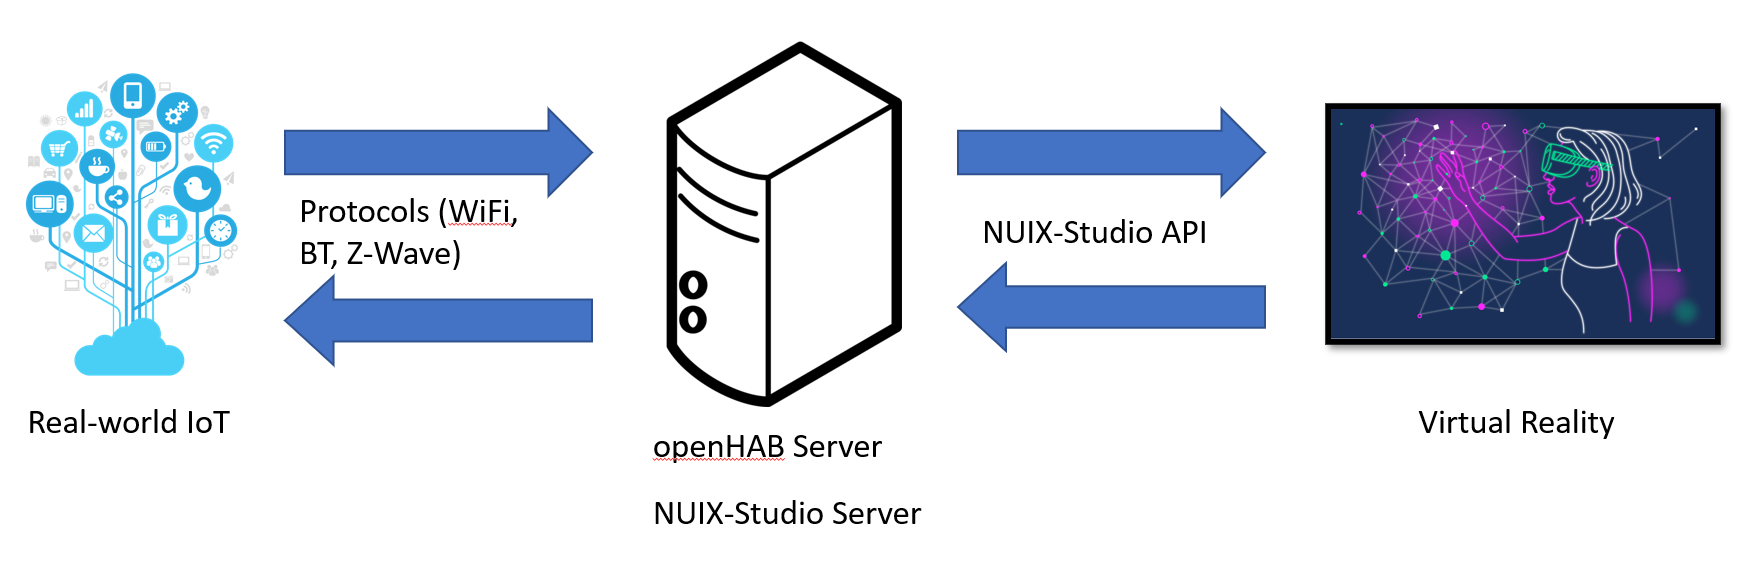
\includegraphics[width=0.6\linewidth]{figures/BasicPlatformStructure.png}
  \caption{Simplified structure of NUIX Studio. Real-world IoT devices HUB is openHAB server, while NUIX-Studio server is the main instance of NUIX-Studio APP responsible for the computations.}
  \label{fig:BasicPlatformStructure-figure}
\end{figure}

\section{Server Architecture}
\subsection{OpenHAB Server Structure}


It was decided not to change the structure of the openHAB system, since it follows the SOA principles that allow to implement support for various types of devices.

Each IoT device is called a Thing, but a Thing can also be a service. For example, a smoke sensor and user location are both Things.

Things expose their capabilities through Channels. For example, a smart vacuum cleaner channels are: suction strength, water delivery strength, remaining charge level, and cleaning status. 

Each channel is associated with one or more Items that are added inside the Model. Items have a State and they may receive commands. 

To add an IoT device to the server, a software adapter should be installed first. These add-ons are called bindings and they provide a way to link Items to physical devices.

\begin{figure}
  \centering
  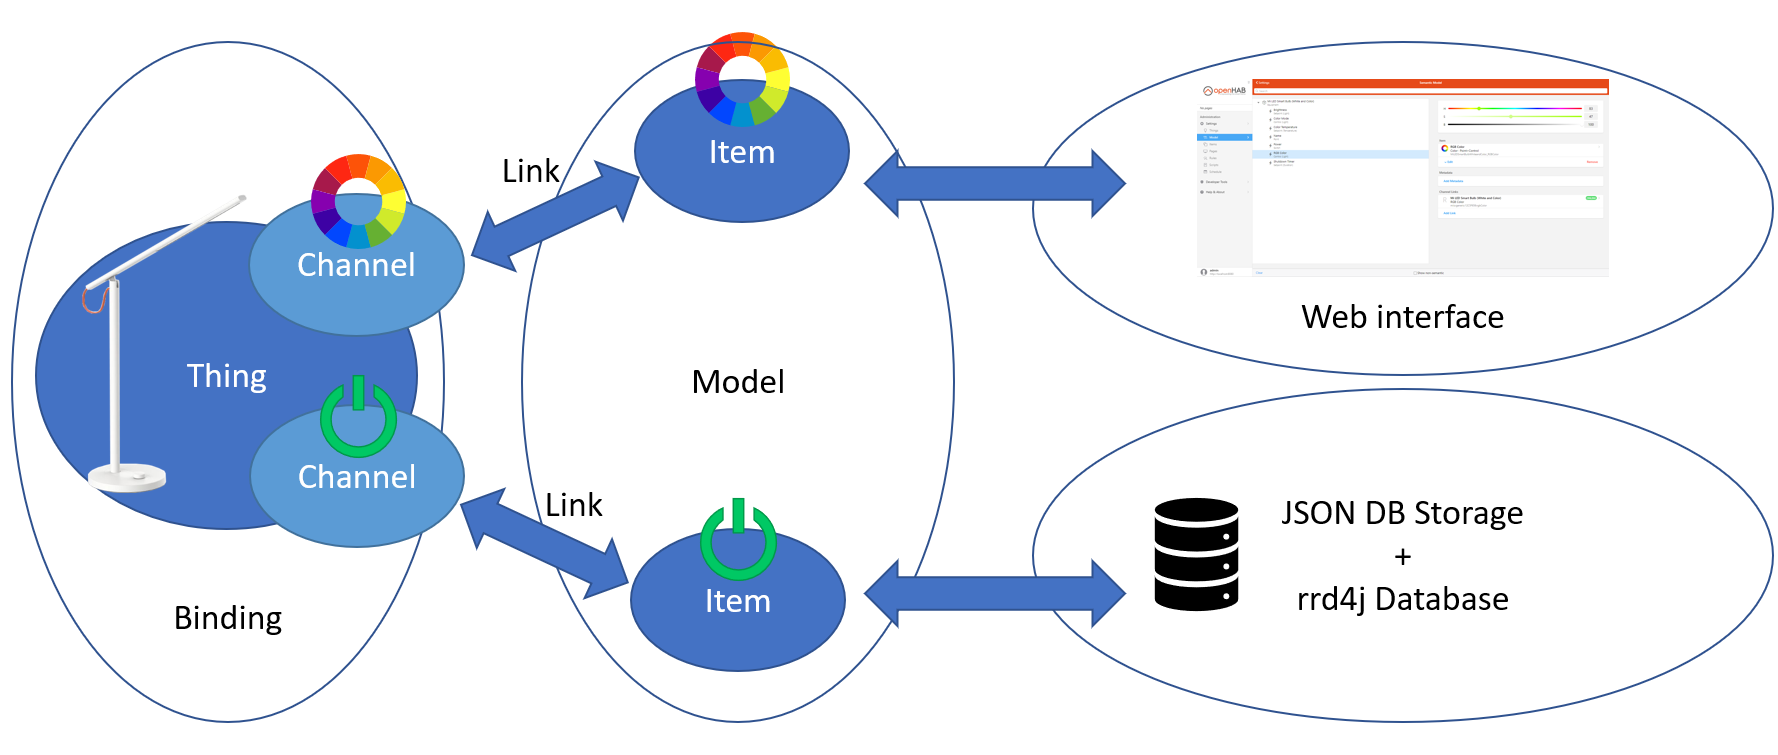
\includegraphics[width=0.9\linewidth]{figures/openHABServerStructure.png}
  \caption{Simplified structure of NUIX Studio. Real-world IoT devices HUB is openHAB server, while NUIX-Studio server is the main instance of NUIX-Studio APP responsible for the computations.}
  \label{fig:openHABServerStructure-figure}
\end{figure}

In the example each of the items is linked only to one channel, and each of the channels is linked to only one item. 

Assume that a binding for Xiaomi smart home devices is installed. The smart home device have been automatically discovered by the server and added as Things. In the example a Xiaomi Lamp is used, for which several Channels are presented (Figure~\ref{fig:XiaomiLampChannels-figure}).

\begin{figure}
  \centering
  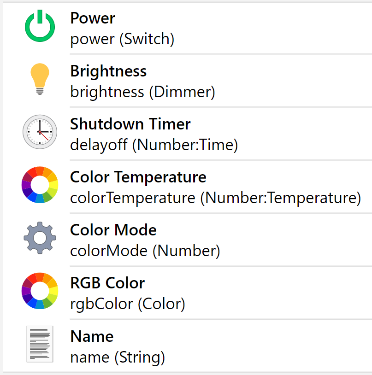
\includegraphics[width=0.6\linewidth]{figures/XiaomiLampChannels.png}
  \caption{Channels list example.}
  \label{fig:XiaomiLampChannels-figure}
\end{figure}

Each of these channels represents one item (Figure~\ref{fig:XiaomiLampPowerItem-figure}).

\begin{figure}
  \centering
  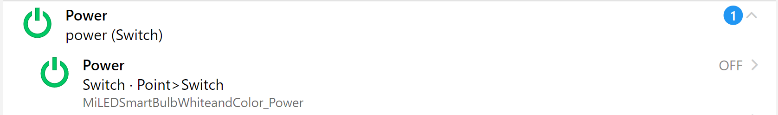
\includegraphics[width=0.9\linewidth]{figures/XiaomiLampPowerItem.png}
  \caption{An Item example.}
  \label{fig:XiaomiLampPowerItem-figure}
\end{figure}

For example, the Power Control is performed through power channel. The Power Control, in terms of the concepts introduced is an item with name MiLEDSmartBulbWhiteandColorPower of type Switch and State “OFF”.

As soon as the lamp is turned On, the Power Control switch in Web Interface will also turn ON. And if the switch is changed to the “OFF” state in the Web Interface, the lamp will turn off.

To support Fault Tolerance, the openHAB server stores data over time.

\subsection{Server Extended Structure}

In the previous paragraph it wasn't specified how the platform should perform access to the server data. 

\begin{figure}
  \centering
  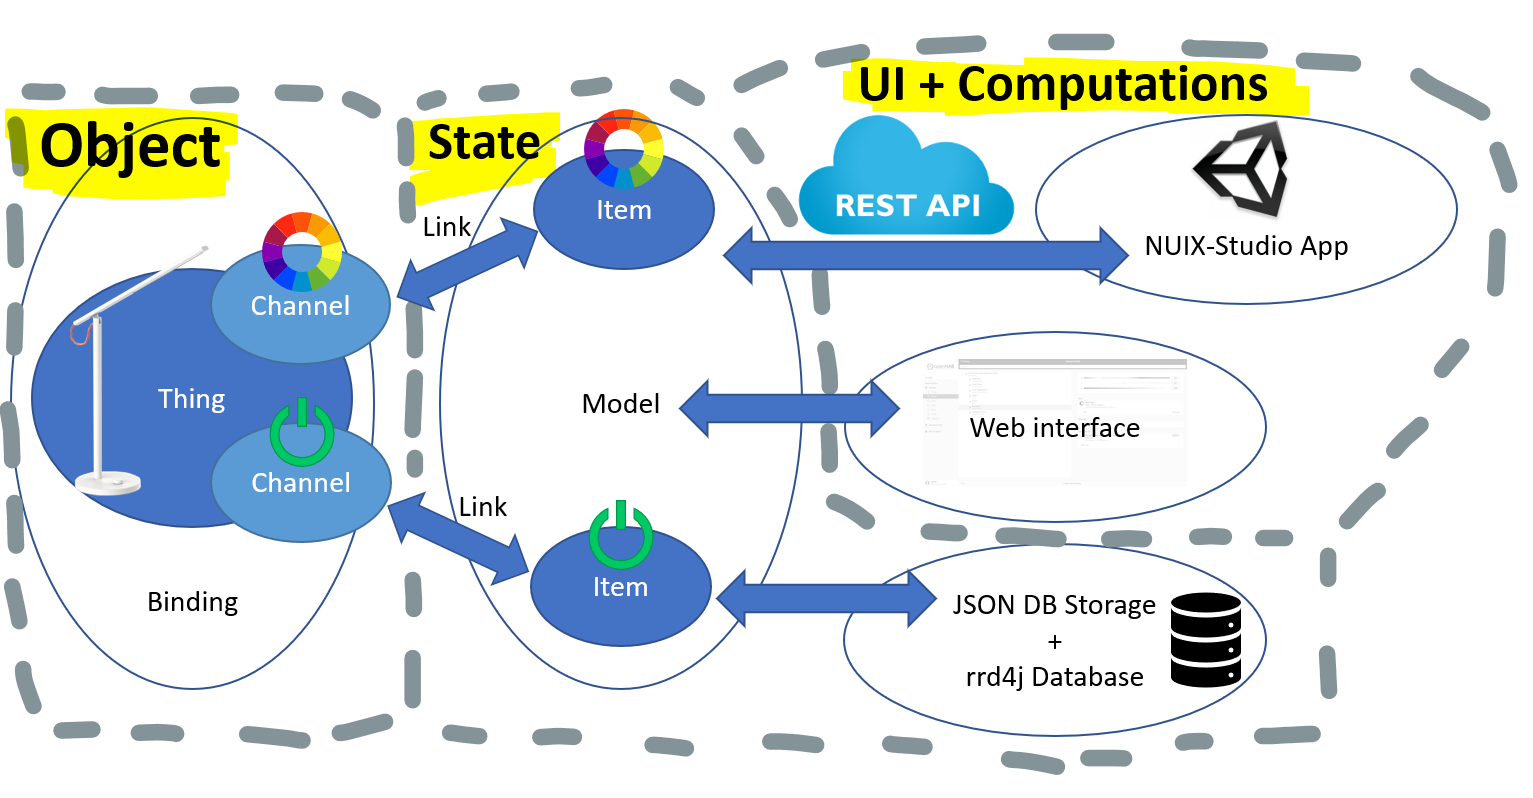
\includegraphics[width=0.9\linewidth]{figures/ExtendedServerStructure.png}
  \caption{Structure of the server showing how the NUIX-Studio APP is connected to it.}
  \label{fig:ExtendedServerStructure-figure}
\end{figure}

As seen on Table~\ref{tab:rest-api-table}, syncing is performed through REST API, which is explained in details further.

\begin{table}
  \centering
  \begin{threeparttable}[c]
    \caption{REST API commands used in NUIX-Studio}
    \label{tab:rest-api-table}
    \begin{tabular}{ll}
      \toprule
      REST API CALL    &         DESCRIPTION                 \\
      \midrule
      GET\tnote{a} & Get all available items \\
      POST\tnote{b} & Adds a new item to the registry or updates the existing item    \\
      PUT\tnote{b}        & Sends a command to the item                              \\
      DELETE\tnote{b}        & Removes an item from the registry          \\
      \bottomrule
    \end{tabular}
    \begin{tablenotes}
      \item [a] For link: /items
      \item [b] For link: /items/<itemname>
    \end{tablenotes}
  \end{threeparttable}
\end{table}

In the current implementation of the platform, 4 different REST API commands are used: GET command for receiving the items in the registry on system startup, PUT command to create a new item on the server, POST command for updating the state of the item, and DELETE command for removing an item from the server.

Receiving the states of the items from the server is performed through getting the events from the server: once the event is received, the item state can be retrieved from payload.

\section{NUIX-Studio APP}

As mentioned above, there can be several NUIX-Studio APP instances running at the same time. Each of them has access and performs syncing to the Server through REST API. The instances can be of one of three types:

\begin{enumerate}
    \item Virtual Reality Instance. Runs on Oculus or another VR headset, has remote or local access to the server. Items received from the server are visualized and it is possible to interact with them using different techniques such as touching buttons, moving sliders, performing gestures using hand recognition, using voice commands etc. 
    \item Computations Instance. Runs on a powerful machine and has either remote or local access to the server. Since latency is important for the VR-IoT platform, it is more preferable to run this instance on the same machine as openHAB. In this case the REST API calls time will be less than minimum measurement unit (compared to milliseconds for accessing remote virtual reality instances). Physics, big data analysis and other performance-based computations are performed on this instance, while interactions are limited.
    \item Input simulation instance. If the APP instance is running on the device with limited support of interaction interfaces (for example, a PC), input simulation can be used. Sometimes, it is even easier to run and test the platform on such devices: for example, if using a physical keyboard is needed, or when there is no access for VR headset at the moment.
\end{enumerate}

\begin{figure}
  \centering
  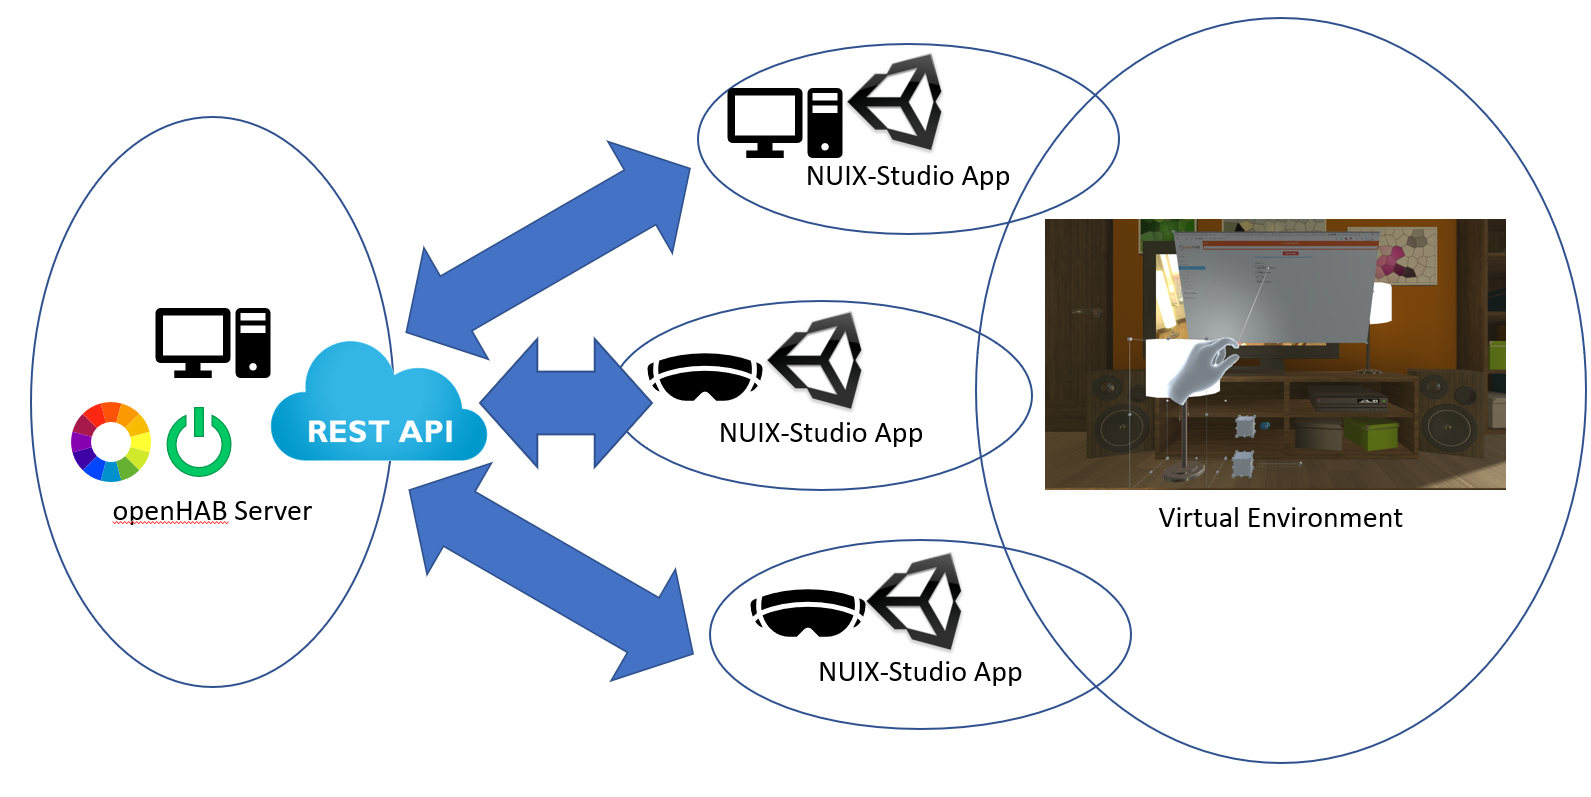
\includegraphics[width=0.9\linewidth]{figures/AppInstances.png}
  \caption{NUIX-Studio App Instances}
  \label{fig:AppInstances-figure}
\end{figure}

Each of the instances performs access to the same data on the server, which makes it possible to work simultaneously in one virtual environment, as well as divide tasks between different instances: as mentioned above, one of the instances can be used for computations, while the other instances for interacting with the devices in Virtual reality.

\subsection{NUIX-Studio App Architecture}

When the NUIX-Studio APP requests the access to the system to get the list of items from the registry, a list of Item Data Transfer Objects is received by the app and then added into Semantic Model. When the state of the item is updated, or if a new item is added or removed, an event is sent to the EventController instance, and then, based on the event payload, the item list in updated.  By keeping each item’s data equal to the server, the semantic model in NUIX-Studio APP is equivalent to the semantic model presented on the server. 

But only keeping the states of the items in the APP does not allow us to interact with the items. In other words, NUIX-Studio App has to provide an interface to interact with the items. Since different types of items require different interaction techniques, for each item type a widget is created.
Widget in NUIX-Studio APP is a Unity Virtual GameObject, which can visualize the item state and update it. For example, it can be an interactable pinch slider for a dimmer item, or a virtual screen  for an image item.

By integrating Extra packages, NUIX-Studio platform can provide a bigger variety of widgets, as well as higher number of supported devices. For example, Oculus Integration support provides an API for hands recognition, while Steam VR support makes it possible to run the NUIX-Studio APP on the majority of VR headsets (Figure~\ref{fig:AppArchitecture-figure}).

\begin{figure}
  \centering
  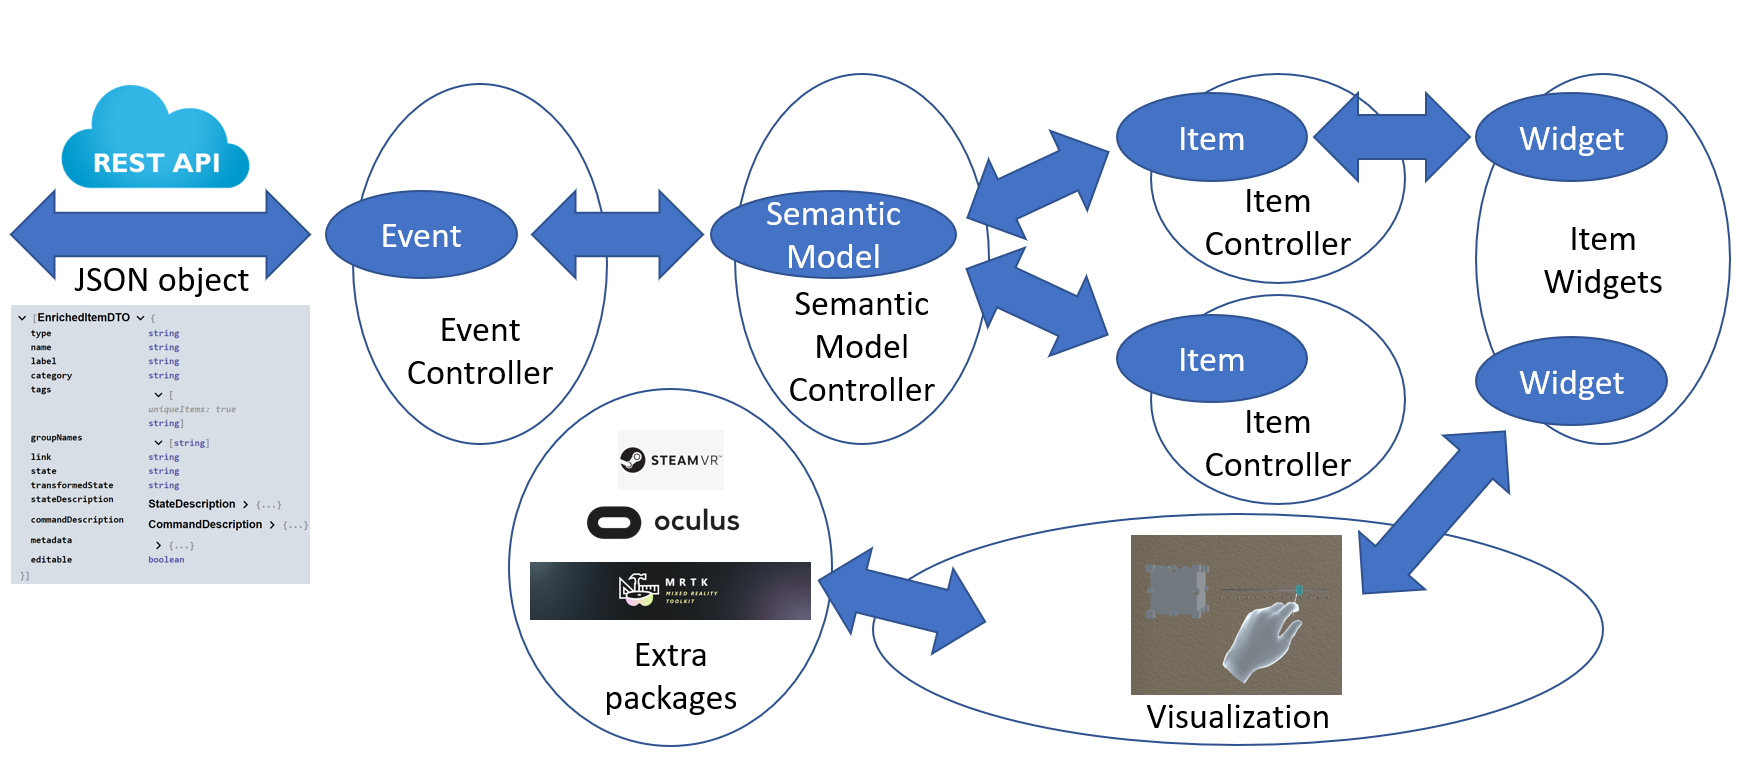
\includegraphics[width=0.9\linewidth]{figures/AppArchitecture.png}
  \caption{NUIX-Studio App Architecture}
  \label{fig:AppArchitecture-figure}
\end{figure}

\subsection{NUIX-Studio APP Semantic Model}

As mentioned above, the semantic model in the NUIX-Studio App is kept equivalent to the semantic model stored on the server. The advantages of this approach are:

\begin{enumerate}
    \item Each of the APP instances visualizes equivalent data, which leads to support of simultaneous and fault-tolerance work;
    \item The semantic model on the server is time and memory effective, and it is better to develop the platform based on such model;
    \item It is more effective solution for using third-party frameworks. Since openHAB is a flexible popular open-source software for IoT systems, in the future, if more functionality is going to used with openHAB, our solution will still be working.
\end{enumerate}

Overall, by using the defined approach, the platform follows Dependency-inversion principle "depend upon abstractions, [not] concretions." In this case, Semantic Model is an abstraction, and Item representation is an abstraction as well.

But in case when it is required to provide an interface for creating new IoT devices in VR and interact with them, it is not possible to use only items presented on the server. For example, the virtual position in the environment for each item is an important data, which should be accessible by each of the instances.

Therefore, the disadvantages of keeping the equivalent semantic models are:

\begin{enumerate}
    \item The semantic model should be extended with extra items, such as virtual position or environment setup. These items are needed by each running instance of NUIX-Studio APP.
    \item The main purpose of the platform is to provide an interface to test new IoT devices inside virtual reality, or extend the existing items with extra functionality. But only real-world devices data is stored on the server, therefore it should be extended with virtual items data.
\end{enumerate}

In result, extending the semantic model with virtual items helps us to minimize the number of disadvantages while keeping the advantages.
In the next chapter an example of using the NUIX-Studio is given and the measured performance is analyzed.